\chapter{Design Project Case Study}
\label{chapter:appendixE}
\graphicspath{ {./appendixE/Fig} }

This appendix contains a highly condensed case study of a capstone
design project that was developed by a team of students utilizing the
principles of this textbook. 

\textbf{The Visual Aid}
Ryan Andrus, Luis Catoni, Carl Schnur, and Freddy Chiu \\
A Senior Project Report Submitted to the Faculty of \\
Electrical, Computer, and Software Engineering \\
Penn State Erie, The Behrend College \\
April 2006

\textbf{1 Problem Statement}\\
\textbf{1.1 Need}


Visually impaired people often have mobility difficulties due to limited
spatial sensing---determining where objects are. Although many receive
education in mobility techniques and enhance other senses to create
better awareness of surroundings, there is a need for a more accurate
spatial description. For example, according to the Vision and Blindness
Resources Center in Erie, visually impaired people are able to detect
walls due to different sounds in the environment. However, a tree
branch, stairs, or a street sign may be undetected. Due to objects that
cannot be perceived by sensorial means, many devices have been designed
to detect objects in the path of a visually impaired individual. Common
mobility resources are guide dogs, canes, and electronic travel aid
(ETA) devices. Unfortunately, these resources are either limited or too
expensive. There is a need for a device to provide an effective way to
detect objects and be cost-efficient.


\textbf{1.2 Objective}\\
The goal is to design and implement a digital system that give visually
impaired an enhanced awareness of their surroundings. The system will
detect objects and provide real-time feedback to the user according to
the size, position, and distance of the object.

\textbf{1.3 Research Survey} \\
For over 30 years, people have been attempting to invent an electronic
device to help the blind navigate. According to the American Foundation
for the Blind {[}1{]}, there are about 10 million blind and visually
impaired individuals in the United States.

According to Seeing Eye {[}2{]}, an organization committed to train dogs
for the blind, around 1\% of the visually impaired use guide dogs. Many
do not choose this option due to allergies, facilities needed for dog
care, training for both the dog and the individual and finally, personal
preference. The rest of the blind community relies on canes, electronic
travel aids (ETA), and their perceptual senses.

The cane is the most popular tool for object detection for the blind.
Nevertheless, this tool is limited as it is difficult to locate objects
that are not at the ground level. For example a tree branch will go
undetected by an individual using a cane. However, there are ETAs
designed to overcome this problem. The most popular ETA is a cane that
contains built-in laser sensors for object detection called the
LaserCane {[}3{]}. This system integrates laser sensors near the handle
of the cane and detects objects in 3 different angles. This system
provides feedback to the user by sound or by vibrations produced on the
side of the cane sensed by touch. Although this design offers the blind
more resources to identify possible objects in front, it has limited
feedback. For instance, the laser sensors fire a beam so narrow that
users must be master the movements of the cane in order to detect
objects accurately. Moreover, this device costs around \$2,500, which
places an attainability issue for many visually impaired.

According to the director of the Vision and Blindness Resources Center
in Erie---whom was interviewed as part of the project's research---the
visually impaired are trained to orient themselves and navigate using
their senses. However, major difficulties arise from objects that cannot
be sensed. Therefore, basic mobility needs of visually impaired consist
of object detection with a range of approximately 1 meter from the body,
as a minimum, and 2 feet wide---the width of the body. Such objects may
include desks, chairs, steps, and tree branches. In an interview with a
visually impaired student on campus who uses a guide dog said that
surface differences of approximately 2 in. should be considered
dangerous, and must be detected by the ETA system.

Based on the needs and common hazards that the visually impaired
encounter, key characteristics must be carefully addressed when
designing an ETA device. First, the sensing system must be able to
detect objects of varied sizes and cover a wide range for ease of
detection. Second, GPS and compasses may be used for orientation. Third,
an intuitive feedback system must be used. Such a system cannot employ
sound as this interferes with the hearing of the visually impaired.
Finally, the system must be affordable. Research shows that no single
device meets all these needs and has been widely accepted by the blind
community.

\textbf{1.4 User Needs and Objective Tree}\\
The team interviewed a number of sources to identify the objectives in
the tree below.

\begin{figure}

\includegraphics[width=3.80278in,height=3.76528in]{./image1.jpeg}
\caption{The needs and objective tree.}
\label{figure:caseStudyNeedsObjective}
\end{figure}

Weightings of the objectives were determined using the pairwise
comparison method for all levels of the objective tree. The results for
the highest level of the tree are portability (0.20), consumer-friendly
(0.30), and ease-of-use (0.50). This result arises from the need that
the ETA must be easy to use because an overly complex interface would
create a high barrier to using and then accepting the device. Along the
same lines the device should create a minimum amount of disturbance to
the user's environment. Finally, while important portability is the
least of the three concerns.


\textbf{2 The Requirements Specification}


\begin{table}
\caption{Requirements Specification for the Visual Aid.}
\label{table:caseStudyRequirements}
\begin{tabular}{|m{3cm}|m{3cm}|m{3cm}|} \hline
\textbf{Marketing Requirements} & \textbf{Engineering Requirements} & \textbf{Justification} \\ \hline

1, 2, 10, 13 & 
		1. The system's total weight will not exceed 5 lbs. & 
		Based on the weight of other portable devices, such as
		laptops, and the weight of book bags. \\ \hline
		
7, 8, 13 & 
		2. The system will have a single control to turn it on/off.  & 
		Based on the user's need for the system to be as simple
		and intuitive as possible and the average person's familiarity with
		technology. \\ \hline
		
5, 13 & 
		3. The system will operate on full charge for at least 3 hours. &
		Based on the expected daily use by considering average
		daily walking time (2.1 miles at 3.3MPH is about 38 minutes/day) by a factor of
		approximately 5. \\ \hline
		
6 & 
		4. The system should not exceed \$600.		&
		Based on the cost of competing products {[}6{]}, such
		as the LaserCane. \\ \hline
		
11 & 
		5. Uneven surfaces (steps, rocks) of at least ±1.25in high will be
		  detected at a distance of at least 3 ft away from the user. &
		Based on the size of possible hazards, such as rocks,
		bottles, sign posts, stairs, etc. \\ \hline
		
11, 14 & 
		6. The system will detect objects that are at least 1in wide and 2in high
		  at a distance of at least 3 ft from the user and as far as 7 ft in an
		  area 2 ft wide, and provide sensory feedback. Also, the system should
		  detect street signs and posts.		&
		Based on the user's need to timely and intuitively be
		notified of hazards. \\ \hline
		
		
12 &
		7. The system should not produce noise exceeding 40dB.	&
		Based on comparisons of sound levels at an office,
		bedroom and living room environment {[}7{]}. \\ \hline

3 & 
		8.  The system will be built with components that can operate in
		  temperatures ranging from 0$^\circ$F to 120$^\circ$F.		&
		Based on the expected range of temperatures the user
		might operate the device in. \\	\hline

3, 4, 9 & 
		9. The system components will be enclosed to be water-resistant.	&
		Based on outdoor environments and its conditions (snow,
		rain, humidity) the user might face and the need for the user to be 
		protected from electrical shock. \\ \hline

14 & 
		10. The system will refresh its output according to sensor readings 5
		  times per second. &
		Based on the average reaction time of humans (0.33 seconds) {[}8{]}. \\ \hline

\multicolumn{3}{l}{
\textbf{Marketing Requirements}
1) Portability, 2) Weight, 3) Operable Environments, 4) Water
Resistant,5)Operation Time, 6) Cost, 7) Ease of use, 8) Streamlined
Controls, 9) Safety, 10) Comfortable, 11) Accurate, 12) Noise Level, 13)
Consumer-Friendly, 14) Intuitive Feedback } \\ \hline

\end{tabular}
\end{table}


\textbf{3 The Design}

The Visual Aid device has three major physical components: 1) a set of
sensors, 2) a matrix of vibrating motors and 3) a processing unit. These
physical components are interconnected through the processing unit and
are attached to the user as in Figure 2 below.


\begin{figure}
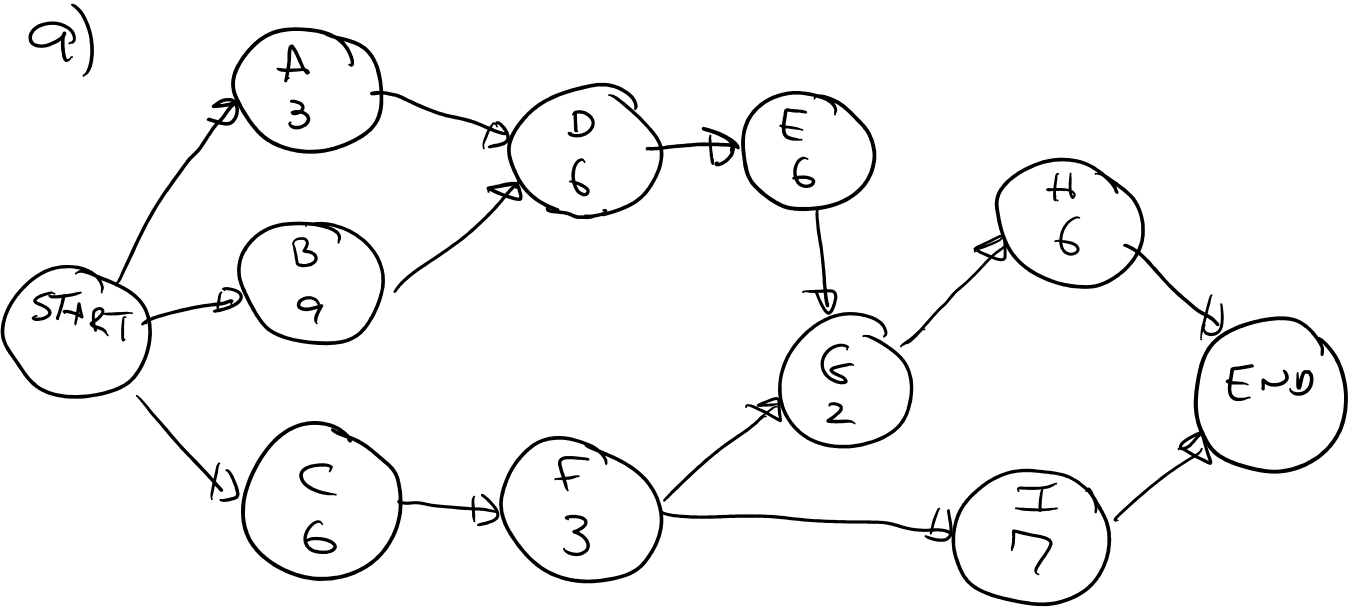
\includegraphics[width=4.93194in,height=3.55278in]{./image2.png}
\caption{Visual Aid side view.}
\label{figure:caseStudySideView}
\end{figure}

The set of sensors is distributed in three modules. The head module
consists of a narrow-beam sensor (represented as a dashed red line)
mounted in the head of the user. The purpose of this module is to
provide the user with accurate information regarding an objects
position, size and distance.

The second module is the array of six wide-beam sensors. The use of
wide-beam sensors enables the system to detect objects in a larger area.
In order to give more detailed information on an object's spatial
location the sensors are arranged such that portions of their beams
overlap with each other. The sensor matrix is aligned to give a wider
range in the vertical orientation than the horizontal.

\begin{figure}
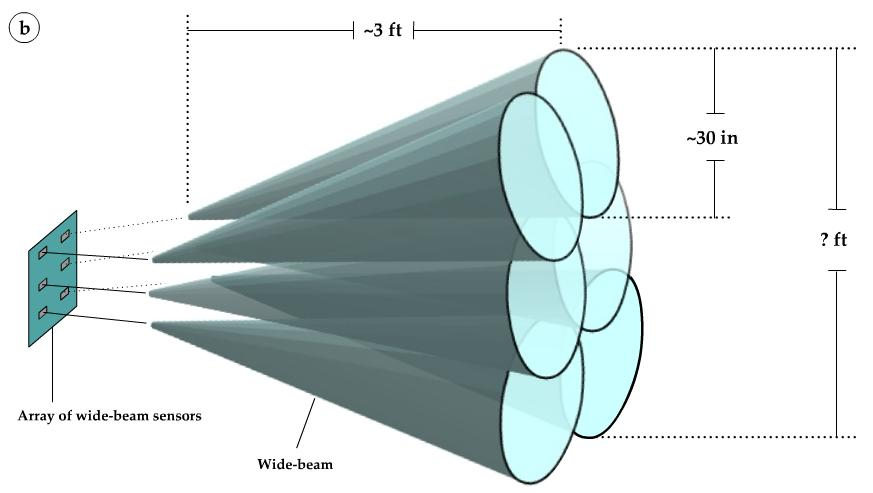
\includegraphics[width=4.50764in,height=2.54514in]{./image3.jpeg}
\caption{Wide-beam sensors array.}
\label{figure:caseStudyWideBeam}
\end{figure}

The third module detects objects and steps up or down at the ground
level. This module consists of a wide-beam sensor and a narrow-beam
sensor. The wide-beam sensor detects objects and obstructions on the
ground. The narrow-beam sensor detects uneven surfaces such as steps and
stairs. This sensor will be positioned as shown in Figure 4 with an
angle $\theta$. This angle is adjustable to fit user needs. On flat surfaces,
the sensor will detect a distance x + z. When a step is encountered, the
distance read by the sensor will be diminished to x. In order to avoid
``false'' detection of steps due to the movement of the user's body
while walking, a digital filter is used.

\begin{figure}
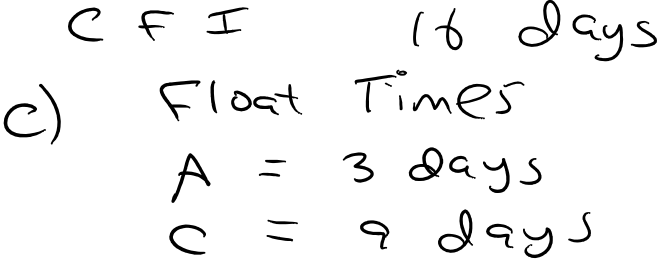
\includegraphics[width=4.25in,height=2.74236in]{./image4.png}
\caption{Narrow-beam sensor.}
\label{figure:caseStudyNarrowBeam}
\end{figure}


The second major component of the system consists of 2 motors located in
the front area of the user (see Figure 5), and 12 vibrating motors
configured in a 3x3 matrix on the back of the user (see Figure 6). The
head unit motor allows the user to scan for objects by moving their
head; the motor will generate higher intensity for closer objects and
lower intensity for farther objects. The narrow-beam motor is used to
provide feedback about an uneven surface detected by the narrow beam
sensor shown in Figure 4. The 3x3 matrix shown in Figure 6 is mounted on
the users back provides feedback according to objects detected in front
of the users. For example if an object is detected in the lower right
corner, then the lower right motor will vibrate. The matrix motors also
vary their intensity according to the distance of objects detected.

\begin{figure}

\includegraphics[width=4.54514in,height=3.04514in]{.//image5.png}
\caption{Sensors and Front Motors}
\label{figure:caseStudySensorMotors}
\end{figure}


\begin{figure}

\includegraphics[width=4.69722in,height=3.09861in]{./image6.png}
\caption{The motors matrix.}
\label{figure:caseStudyMotorMatrix}
\end{figure}

The array of motors is mounted on the user with a vest. The array of
sensors is located on the user's chest and the motor matrix are located
on the user's back. The last physical component is the processing unit.
This consists of the microcontroller unit which will read the inputs
from all the sensors and will provide corresponding outputs to the user
by controlling the vibrating motors.


\textbf{3.1 The Functional Decomposition}


The following sections outline the decomposition of level 0 diagram into
a level 1 diagram with the design rationale included to provide some
justification for the decisions made.



\textbf{Level 0}

The level 0 description of the Visual Aide describes the overall input,
output, and behavior expected of the device.

\begin{figure}

\includegraphics[width=3.53056in,height=2.45486in]{./image7.png}
\caption{Level 0.}
\label{figure:caseStudyLevel0}
\end{figure}


The rationale for our level 0 design was to keep the system easy to
control by a non-technical user. Too many buttons would confuse the
user. The system will take environmental data of the surroundings
(objects) as input and provide vibration feedback as output to the user.
The only control is an on/off switch with everything else automated. The
object is to provide the user with care-free operation.


\begin{table}

\label{table:caseStudyLevel0}
\begin{tabular}{|m{3cm}|m{10cm}|} \hline

\emph{Module} & Vision System \\ \hline

\emph{Inputs} & - User control: on/off
- Environment (objects): objects at least 1 in. wide and 2 in. high
found in a 2 ft. wide area in front of the user, including steps. \\ \hline

\emph{Outputs} & - Sensorial feedback (vibrations): a 3x3 matrix of
vibrating motors, plus three additional vibrating motors. \\ \hline

\emph{Functionality} & Alerts the user intuitively by means of vibrating
motors as to what area and distance in front of the user object(s)
is(are) and/or if there is a step. Detected objects are at least 1 in.
wide and 2 in. high at a distance of at least 3 ft. from the user and as
far as 7 ft. in an area 2 ft. wide. Variations of height (steps, rocks)
of at least ±1.25 in. are detected at a distance of at least 3 ft. away
from the user. \\ \hline
\end{tabular}
\end{table}

\textbf{Level 1}

The level 1 diagram reveals what is inside the level 0 box shown in
Figure~\ref{figure:caseStudyLevel0}.

\begin{figure}
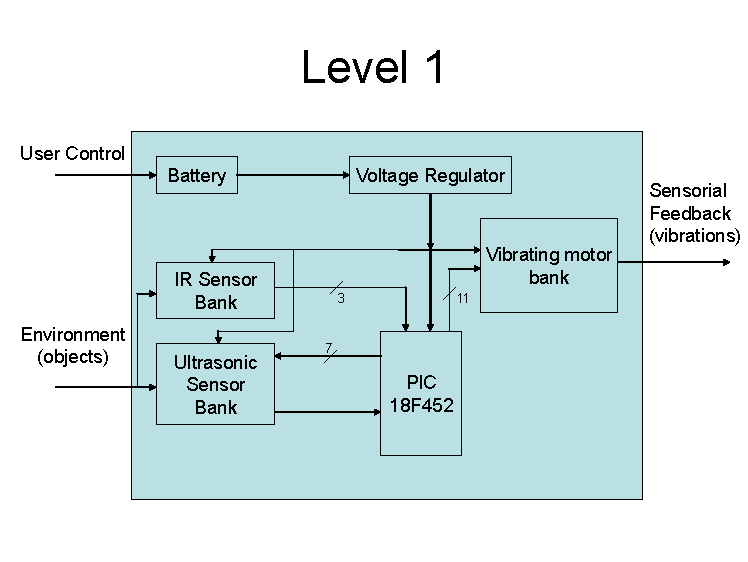
\includegraphics{./image8}
\caption{ Level 1 system design.}
\label{figurecaseStudyLevel1:}
\end{figure}


There are four main components in this part of our system design: the IR
sensor bank, ultrasonic sensor bank, PIC18F452, and vibrating motor
bank. Also, there are modules for supplying power to the components such
as a voltage regulator.

The reason for breaking the design into these four main components is
because each one provides a separate and distinct functionality towards
the overall operation of the system. The IR Sensor Bank is responsible
for detecting changes in elevation of the surface (steps, curbs, ledges)
and also to identify objects targeted by they user's head. The
Ultrasonic Sensor Bank is responsible for detecting objects directly in
front of the user and also indicating the object's general location. The
PIC18F452 is the control unit of the entire system. It will read data
from the sensor banks, process the data, and provide feedback control
via the vibrating motor bank. Finally, the vibrating motor bank, which
is mounted on the back of the user, provides sensorial feedback to the
user in the form of vibrations of varying intensity based on the
proximity of the object and relative to the location of the object.

\begin{table}
\begin{tabular}{|m{2cm}|m{10cm}|} \\ \hline
\emph{Module} & Battery \\ \hline
\emph{Inputs} & - User control: on/off \\ \hline
\emph{Outputs} & - 9.6V DC \\ \hline
\emph{Functionality} & Provide power to all electronics in the system. \\ \hline
\end{tabular}
\end{table}


\begin{table}
\begin{tabular}{|m{2cm}|m{10cm}|} \\ \hline
\emph{Module} & Voltage Regulator \\  \hline
\emph{Inputs} & - 9.6V DC \\ \hline
\emph{Outputs} & - 5V DC with up to 1A of current. \\ \hline
\emph{Functionality} & Convert the battery's 9.6V DC to 5V DC. \\ \hline
\end{tabular}
\end{table}

\begin{table}
\begin{tabular}{|m{2cm}|m{10cm}|} \\ \hline
\emph{Module} & IR Sensor Bank \\ \hline
\emph{Inputs} & - 5V DC for power. 
- Environment (objects): objects at head level and steps. \\ \hline
\emph{Outputs} & - V\textsubscript{0}-V\textsubscript{2}: voltages ranging from 0.55V DC to 2.8V DC \\ \hline
\emph{Functionality} & One sensor to detect objects at head level and
another sensor angled to detect uneven surfaces. \\ \hline
\end{tabular}
\end{table}

\begin{table}
\begin{tabular}{|m{2cm}|m{10cm}|} \\ \hline
\emph{Module} & Ultrasonic Sensor Bank \\ \hline
\emph{Inputs} & - 5V DC for power.
- Environment (objects): objects at least 1in wide and 2in high found in
a 2ft wide area in front of the user.

- D\textsubscript{0}-D\textsubscript{7}: forwarded 5V DC 10µs control
signal from PIC to selected sensor. \\ \hline
\emph{Outputs} & - U\textsubscript{0}-U\textsubscript{7}: 0-5V DC pulse
signal from 100µs to 18ms corresponding to selected sensor. \\ \hline
\emph{Functionality} & Detects objects on the floor and in front of the
user (under head level), and gives feedback regarding location and
distance to object. \\ \hline
\end{tabular}
\end{table}

\begin{table}
\begin{tabular}{|m{2cm}|m{10cm}|} \\ \hline
\emph{Module} & Vibrating Motor Bank \\ \hline
\emph{Inputs} & - 5V DC for power.
- M\textsubscript{0}-M\textsubscript{11}: PWM signals from 0-5V DC \\ \hline
\emph{Outputs} & - Sensorial feedback (vibrations): sustained or pulsed
vibrations with varied intensities. \\ \hline
\emph{Functionality} & Converts the processed sensor information into
feedback for the user. \\ \hline
\end{tabular}
\end{table}

\begin{table}
\begin{tabular}{|m{2cm}|m{10cm}|} \\ \hline
\emph{Module} & PIC 18F452 \\ \hline
\emph{Inputs} & - 5V DC for power.
- R\textsubscript{0}-R\textsubscript{2}: analog voltage feedback from
0.55Vto 2.8V
- U\textsubscript{X}: 0-5V DC pulse signal from 100µs to 18ms. \\ \hline
\emph{Outputs} & - S\textsubscript{0}-S\textsubscript{2}: digital select
lines
- U\textsubscript{C}: 5V DC 10µs pulse
- M\textsubscript{0}-M\textsubscript{11}: PWM signals with \ul{?} period
and \ul{?}\% duty cycle \\ \hline
\emph{Functionality} & Gather data from ultrasonic and IR sensors, then
convert it to PWM signals that drive the vibrating motors. \\ \hline
\end{tabular}
\end{table}

The first decision for the design was which method was best to detect
objects. The following table outlines some of the advantages and
disadvantages of a few methods.


\begin{table}
\caption{Sensor selection decision.}
\label{table:caseStudySensorDecision}
\begin{tabular}{|m{4cm}|m{4cm}|m{4cm}|} \hline
\emph{\textbf{Method}} & \emph{\textbf{Advantages}} & \emph{\textbf{Disadvantages}} \\ \hline
Ultrasonic sensor & Wide range Inexpensive & Less accurate \\ \hline
IR sensor & Accurate Inexpensive & Limited scope and range \\ \hline
Lasers & Accurate Long distance detection & Expensive Limited scope \\ \hline
Radar & Infinite range Near perfect accuracy & Very expensive Large and heavy Expert knowledge required \\ \hline
\end{tabular}
\end{table}

Ultrasonic sensors were capable of detecting the area which we required
(Range: 1'' -- 10', with area of detection growing wider as distance
increases). Infrared sensors were chosen because they have a relatively
narrow beam which can be used to easily pinpoint the location of an
object and also to conduct precise measurements to changes in elevation.

The main disadvantages to laser and radar technology were high costs and
bulkiness. Also, no group member is familiar with the technology and
large amounts of time to learn would be required. Laser technology is
useful in detecting small objects at far distances, but we found that
the large range of the lasers was unnecessary and the price of this
technology is too high.

The next decision falls in the category of feedback to the user. The
following table outlines of the advantages and disadvantages of two
methods.

\begin{table}
\caption{ser feedback selection.}
\label{table:<context>}
\begin{tabular}{|m{3cm}|m{3cm}|m{3cm}|} \hline
\emph{\textbf{Method}} & \emph{\textbf{Advantages}} & \emph{\textbf{Disadvantages}} \\ \hline
Vibration & Quiet operation Inexpensive & May take time for user to get used to this type of
sensorial feedback \\ \hline
Audible & Unlimited capability & Interferes with a blind user's vital
hearing ability \\ \hline
\end{tabular}
\end{table}

The two alternatives to choose from involving feedback to the user were
either through vibrations or audible sounds. After some interviews and
extensive research of the visually-impaired, we learned that audible
feedback would interfere with their vital sense of hearing. Most blind
people are trained to enhance their hearing capability to navigate
naturally as they walk so they typically avoid using devices that
produce audible feedback. We chose to use the vibration method due to
its quiet operation, although this method will likely require some
getting used to as people are not used to having things producing this
type of sensorial feedback on their body.

Finally, we needed to choose a method to control the other 3 components
of the design. We chose the PIC18F452 because it provides subsystems
that are very useful for our design such as multiple timer modules, and
an ADC subsystem. Also, our familiarity with this device encouraged us
to use it for our main control. The PIC also provides many I/O ports,
plenty of internal flash memory, and is an inexpensive device.


 \textbf{3.2 High Level Software Description}

The development of the software system exhibits the same modularity as
the hardware design shown in Figure~\ref{figurecaseStudyLevel1:}. 
Figure~\ref{figure:caseStudySoftwareArch} shows the overall
behavior of the system as a state diagram, listing out the sequence of
operations that are performed by the MCU.

\begin{figure}

\includegraphics{./image9}
\caption{Main state diagram for software.}
\label{figure:caseStudySoftwareArch}
\end{figure}

In the list that follows, each of the states in 
Figure~\ref{figure:caseStudySoftwareArch} is described in
more details regarding its functionality.

\begin{itemize}
\item
  \textbf{Start -} This is a dummy state to represent the system when it
  is turned on. It will transition to Initialize Hardware state.
\item
  \textbf{Initialize -} This is a function that runs at the beginning of
  the program (upon power-up of the system) to initialize the different
  hardware and modules used.
\item
  \textbf{Check Floor Sensor Value Read -} The values read from the
  floor unit, specifically the narrow-beam sensor, are used to determine
  whether an uneven surface has been detected or not. If the surface is
  uneven, activate the corresponding motor.
\item
  \textbf{Check Head Sensor Value Read -} The values read from the head
  unit are used to determine and set intensity that the motor
  corresponding to this unit should operate.
\item
  \textbf{Pulse Wide-Beam Sensors -} This calls a function to pulse the
  ultrasonic sensors.
\item
  \textbf{Check Wide-Beam Sensors Value Read -} The values from the
  ultrasonic sensors are used to determine where objects are and to
  activate the corresponding motors.
\item
  \textbf{Interrupt -} This is a state to represent the various
  interrupt that can occur during the program. The only state where the
  interrupts are deactivated is in the Check Wide-Beam Sensors Value
  Read state. They have been deactivated due to sensitivity in the
  program to determine the pattern in which motors should be vibrating.
\end{itemize}


\textbf{4 Design Verification and Testing}


The design testing is presented in the order that the tests were
performed, from unit to acceptance tests.

\textbf{4.1 Unit Testing}

The performance of the IR sensor was critical to the success of the
system as it would be observing the floor and informing the user of any
upcoming steps. We had to test the sensor to see if it could distinguish
the height bob of a walker from the drop off of a set of steps.

\textbf{Table 7}---IR sensor test.

\begin{longtable}[]{@{}
  >{\raggedright\arraybackslash}p{(\columnwidth - 12\tabcolsep) * \real{0.0814}}
  >{\raggedright\arraybackslash}p{(\columnwidth - 12\tabcolsep) * \real{0.4525}}
  >{\raggedright\arraybackslash}p{(\columnwidth - 12\tabcolsep) * \real{0.0679}}
  >{\raggedright\arraybackslash}p{(\columnwidth - 12\tabcolsep) * \real{0.0679}}
  >{\raggedright\arraybackslash}p{(\columnwidth - 12\tabcolsep) * \real{0.0455}}
  >{\raggedright\arraybackslash}p{(\columnwidth - 12\tabcolsep) * \real{0.0224}}
  >{\raggedright\arraybackslash}p{(\columnwidth - 12\tabcolsep) * \real{0.2624}}@{}}
\toprule\noalign{}
\multicolumn{5}{@{}>{\raggedright\arraybackslash}p{(\columnwidth - 12\tabcolsep) * \real{0.7152} + 8\tabcolsep}}{%
\begin{minipage}[b]{\linewidth}\raggedright
\textbf{Test Name:} IR Sensor Test
\end{minipage}} &
\multicolumn{2}{>{\raggedright\arraybackslash}p{(\columnwidth - 12\tabcolsep) * \real{0.2848} + 2\tabcolsep}@{}}{%
\begin{minipage}[b]{\linewidth}\raggedright
\textbf{Test Number:} 101
\end{minipage}} \\
\midrule\noalign{}
\endhead
\bottomrule\noalign{}
\endlastfoot
\multicolumn{7}{@{}>{\raggedright\arraybackslash}p{(\columnwidth - 12\tabcolsep) * \real{1.0000} + 12\tabcolsep}@{}}{%
\textbf{Test Description:} Verify that the IR sensor is correctly
reading distance without unnecessary noise.} \\
\multicolumn{7}{@{}>{\raggedright\arraybackslash}p{(\columnwidth - 12\tabcolsep) * \real{1.0000} + 12\tabcolsep}@{}}{%
\textbf{Test Information}} \\
\multicolumn{2}{@{}>{\raggedright\arraybackslash}p{(\columnwidth - 12\tabcolsep) * \real{0.5339} + 2\tabcolsep}}{%
\textbf{Name of Tester: Luis}} &
\multicolumn{4}{>{\raggedright\arraybackslash}p{(\columnwidth - 12\tabcolsep) * \real{0.2036} + 6\tabcolsep}}{%
\textbf{Date: 3/18/06}} & \textbf{Time: 2:00PM} \\
\textbf{\#} & \textbf{Procedure} & \textbf{Pass} & \textbf{Fail} &
\multicolumn{2}{>{\raggedright\arraybackslash}p{(\columnwidth - 12\tabcolsep) * \real{0.0679} + 2\tabcolsep}}{%
\textbf{N/A}} & \textbf{Comments} \\
\textbf{1} & Mount the IR Sensor and hold it vertically at waist level.
& \textbf{x} & &
\multicolumn{2}{>{\raggedright\arraybackslash}p{(\columnwidth - 12\tabcolsep) * \real{0.0679} + 2\tabcolsep}}{%
} & \\
\textbf{2} & Start Recording data while walking along a flat,
obstacle-free path. & \textbf{x} & &
\multicolumn{2}{>{\raggedright\arraybackslash}p{(\columnwidth - 12\tabcolsep) * \real{0.0679} + 2\tabcolsep}}{%
} & \\
\textbf{3} & Analyze that data to ensure that minimal noise is created
from the up and down movement of walking. & \textbf{x} & &
\multicolumn{2}{>{\raggedright\arraybackslash}p{(\columnwidth - 12\tabcolsep) * \real{0.0679} + 2\tabcolsep}}{%
} & Used Luis, Carl, and a rolling cart. \\
\textbf{4} & Repeat test with stairs along the walking path. &
\textbf{x} & &
\multicolumn{2}{>{\raggedright\arraybackslash}p{(\columnwidth - 12\tabcolsep) * \real{0.0679} + 2\tabcolsep}}{%
} & \\
\textbf{5} & Analyze the values to ensure that they differ enough from
data along the flat surface. & \textbf{x} & &
\multicolumn{2}{>{\raggedright\arraybackslash}p{(\columnwidth - 12\tabcolsep) * \real{0.0679} + 2\tabcolsep}}{%
} & See data on next page for plots with different filters used. \\
\end{longtable}

\begin{figure}
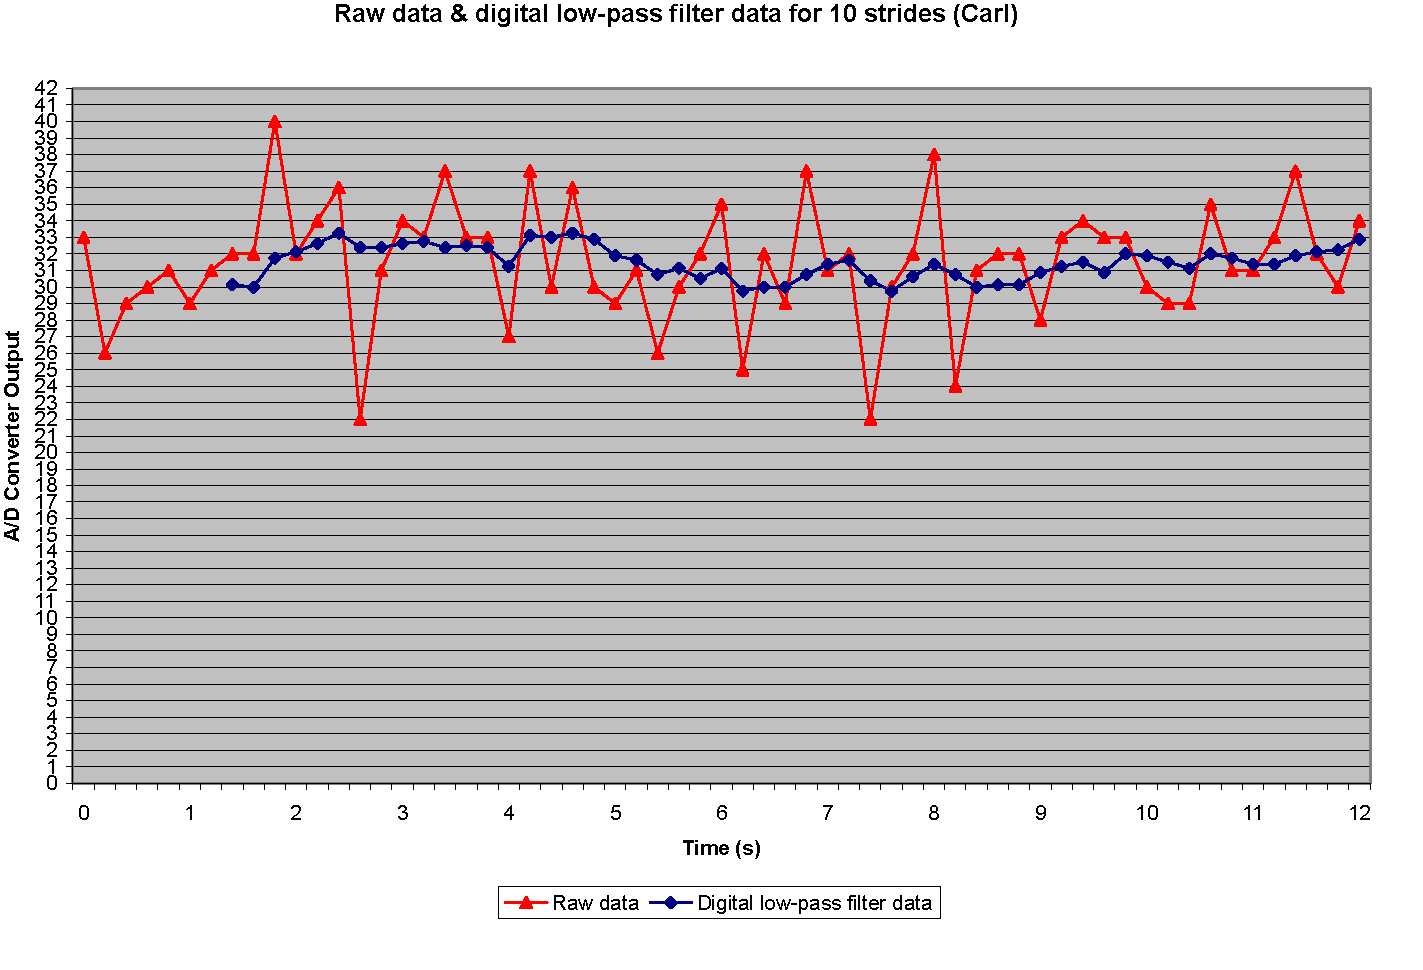
\includegraphics[width=5.44722in,height=3.71181in]{./image10}
\caption{ ADC samples from the narrow beam sensor, raw and filtered.}
\label{figure:caseStudyAdcSamples}
\end{figure}

The graph above shows the effects of using a digital low-pass filter on
the readings from an IR sensor mounted at stomach-level on a walking
person. The person walked on an even surface in a laboratory environment
to gather the data samples. In comparison with the data obtained from
the cart, the raw data has more noise, yet the low-pass filter manages
to stabilize the value considerably.


\textbf{4.1.1 Integration Testing}

This integration test checks that individual ultrasonic sensors could
trigger individual motors. This is critical to insuring that the system
gives proper feedback to the user about their environment.

\textbf{Table 8} -- Integration testing

\begin{longtable}[]{@{}
  >{\raggedright\arraybackslash}p{(\columnwidth - 12\tabcolsep) * \real{0.0845}}
  >{\raggedright\arraybackslash}p{(\columnwidth - 12\tabcolsep) * \real{0.4695}}
  >{\raggedright\arraybackslash}p{(\columnwidth - 12\tabcolsep) * \real{0.0704}}
  >{\raggedright\arraybackslash}p{(\columnwidth - 12\tabcolsep) * \real{0.0704}}
  >{\raggedright\arraybackslash}p{(\columnwidth - 12\tabcolsep) * \real{0.0472}}
  >{\raggedright\arraybackslash}p{(\columnwidth - 12\tabcolsep) * \real{0.0232}}
  >{\raggedright\arraybackslash}p{(\columnwidth - 12\tabcolsep) * \real{0.2347}}@{}}
\toprule\noalign{}
\multicolumn{5}{@{}>{\raggedright\arraybackslash}p{(\columnwidth - 12\tabcolsep) * \real{0.7420} + 8\tabcolsep}}{%
\begin{minipage}[b]{\linewidth}\raggedright
\textbf{Test Name:} Ultrasonic Sensor/Motor Test
\end{minipage}} &
\multicolumn{2}{>{\raggedright\arraybackslash}p{(\columnwidth - 12\tabcolsep) * \real{0.2580} + 2\tabcolsep}@{}}{%
\begin{minipage}[b]{\linewidth}\raggedright
\textbf{Test Number:} 200
\end{minipage}} \\
\midrule\noalign{}
\endhead
\bottomrule\noalign{}
\endlastfoot
\multicolumn{7}{@{}>{\raggedright\arraybackslash}p{(\columnwidth - 12\tabcolsep) * \real{1.0000} + 12\tabcolsep}@{}}{%
\textbf{Test Description:}} \\
\multicolumn{7}{@{}>{\raggedright\arraybackslash}p{(\columnwidth - 12\tabcolsep) * \real{1.0000} + 12\tabcolsep}@{}}{%
\textbf{Test Information}} \\
\multicolumn{2}{@{}>{\raggedright\arraybackslash}p{(\columnwidth - 12\tabcolsep) * \real{0.5540} + 2\tabcolsep}}{%
\textbf{Name of Tester: Freddy and Ryan}} &
\multicolumn{4}{>{\raggedright\arraybackslash}p{(\columnwidth - 12\tabcolsep) * \real{0.2113} + 6\tabcolsep}}{%
\textbf{Date: 3/25/06}} & \textbf{Time: 1:00PM} \\
\textbf{\#} & \textbf{Procedure} & \textbf{Pass} & \textbf{Fail} &
\multicolumn{2}{>{\raggedright\arraybackslash}p{(\columnwidth - 12\tabcolsep) * \real{0.0704} + 2\tabcolsep}}{%
\textbf{N/A}} & \textbf{Comments} \\
\textbf{1} & The tester should be wearing the visual aid system with the
ultrasonic sensors and vibrating motors properly installed. & \textbf{x}
& &
\multicolumn{2}{>{\raggedright\arraybackslash}p{(\columnwidth - 12\tabcolsep) * \real{0.0704} + 2\tabcolsep}}{%
} & \\
\textbf{2} & Have someone place and object in the path of each
individual sensor. & \textbf{x} & &
\multicolumn{2}{>{\raggedright\arraybackslash}p{(\columnwidth - 12\tabcolsep) * \real{0.0704} + 2\tabcolsep}}{%
} & \\
\textbf{3} & Verify that the user is able to identify which position on
the vibrating motor bank is being activated. Also, ensure the correct
motor is being activated. & \textbf{x} & &
\multicolumn{2}{>{\raggedright\arraybackslash}p{(\columnwidth - 12\tabcolsep) * \real{0.0704} + 2\tabcolsep}}{%
} & \\
\textbf{4} & Repeat step (3) for each ultrasonic sensor combination in
order to activate each vibrating motor separately. & \textbf{x} & &
\multicolumn{2}{>{\raggedright\arraybackslash}p{(\columnwidth - 12\tabcolsep) * \real{0.0704} + 2\tabcolsep}}{%
} & \\
\textbf{5} & Next, repeat the same procedure but activate multiple
ultrasonic sensors and vibrating motors simultaneously and ensure that
the unit is functioning properly. & \textbf{x} & &
\multicolumn{2}{>{\raggedright\arraybackslash}p{(\columnwidth - 12\tabcolsep) * \real{0.0704} + 2\tabcolsep}}{%
} & See conclusions below. \\
\end{longtable}

This testing was performed many times and helped us to determine the
proper adjustments/angles of the sensors. Performing these tests also
gave us insight on what to set the sensor thresholds at in the software.

\textbf{4.1.2 Acceptance Testing}
\end{enumerate}

One of the main engineering requirements is \emph{The system will detect
objects that are at least 1in wide and 2in high at a distance of at
least 3 ft from the user and as far as 7 ft in an area 2 ft wide, and
provide sensory feedback. Also, the system should detect street signs
and posts.} In order to insure that this requirement was met, the
following acceptance test was constructed.

\textbf{Table 9} -- Surface test.

\begin{longtable}[]{@{}
  >{\raggedright\arraybackslash}p{(\columnwidth - 12\tabcolsep) * \real{0.0732}}
  >{\raggedright\arraybackslash}p{(\columnwidth - 12\tabcolsep) * \real{0.4065}}
  >{\raggedright\arraybackslash}p{(\columnwidth - 12\tabcolsep) * \real{0.0610}}
  >{\raggedright\arraybackslash}p{(\columnwidth - 12\tabcolsep) * \real{0.0610}}
  >{\raggedright\arraybackslash}p{(\columnwidth - 12\tabcolsep) * \real{0.0409}}
  >{\raggedright\arraybackslash}p{(\columnwidth - 12\tabcolsep) * \real{0.0201}}
  >{\raggedright\arraybackslash}p{(\columnwidth - 12\tabcolsep) * \real{0.3374}}@{}}
\toprule\noalign{}
\multicolumn{5}{@{}>{\raggedright\arraybackslash}p{(\columnwidth - 12\tabcolsep) * \real{0.6425} + 8\tabcolsep}}{%
\begin{minipage}[b]{\linewidth}\raggedright
\textbf{Test Name:} Object Detection Test
\end{minipage}} &
\multicolumn{2}{>{\raggedright\arraybackslash}p{(\columnwidth - 12\tabcolsep) * \real{0.3575} + 2\tabcolsep}@{}}{%
\begin{minipage}[b]{\linewidth}\raggedright
\textbf{Test Number:} 305
\end{minipage}} \\
\midrule\noalign{}
\endhead
\bottomrule\noalign{}
\endlastfoot
\multicolumn{7}{@{}>{\raggedright\arraybackslash}p{(\columnwidth - 12\tabcolsep) * \real{1.0000} + 12\tabcolsep}@{}}{%
\textbf{Test Description:} Verify that the system can detect objects
that are at least 1in wide and 2in high at a distance of at least 3 ft
from the user and as far as 7 ft in an area 2 ft wide, and provide
sensory feedback. Also, the system should detect street signs and
posts} \\
\multicolumn{7}{@{}>{\raggedright\arraybackslash}p{(\columnwidth - 12\tabcolsep) * \real{1.0000} + 12\tabcolsep}@{}}{%
\textbf{Test Information}} \\
\multicolumn{2}{@{}>{\raggedright\arraybackslash}p{(\columnwidth - 12\tabcolsep) * \real{0.4797} + 2\tabcolsep}}{%
\textbf{Name of Tester: Freddy and Ryan}} &
\multicolumn{4}{>{\raggedright\arraybackslash}p{(\columnwidth - 12\tabcolsep) * \real{0.1829} + 6\tabcolsep}}{%
\textbf{Date: 3/18/06}} & \textbf{Time: 12:30PM} \\
\textbf{\#} & \textbf{Procedure} & \textbf{Pass} & \textbf{Fail} &
\multicolumn{2}{>{\raggedright\arraybackslash}p{(\columnwidth - 12\tabcolsep) * \real{0.0610} + 2\tabcolsep}}{%
\textbf{N/A}} & \textbf{Comments} \\
\textbf{1} & On a flat level surface first mark a spot which is where
the system will take readings from. & \textbf{x} & &
\multicolumn{2}{>{\raggedright\arraybackslash}p{(\columnwidth - 12\tabcolsep) * \real{0.0610} + 2\tabcolsep}}{%
} & \\
\textbf{2} & Next, mark out a rectangular box on the floor, starting 3
feet from the testing position. The box should be centered with the
testing spot and be 2 feet wide and 4 feet long. This box is used as
reference for placing objects. (See comments) & \textbf{X} & &
\multicolumn{2}{>{\raggedright\arraybackslash}p{(\columnwidth - 12\tabcolsep) * \real{0.0610} + 2\tabcolsep}}{%
} & 3'

2'

4'

\textbf{X} \\
\textbf{3} & Place a small object which is approximately 1'' wide and
2'' high across the front line (Left Corner, Right Corner and Middle).
Verify that the object is detected at each position and the appropriate
motors are activated. & \textbf{X} & &
\multicolumn{2}{>{\raggedright\arraybackslash}p{(\columnwidth - 12\tabcolsep) * \real{0.0610} + 2\tabcolsep}}{%
} & x x x \\
\textbf{4} & Now, repeat step (3) but place the object across the back
line. & \textbf{X} & &
\multicolumn{2}{>{\raggedright\arraybackslash}p{(\columnwidth - 12\tabcolsep) * \real{0.0610} + 2\tabcolsep}}{%
} & x x x \\
\textbf{5} & Again, repeat step (3) but place the object across the
center of the box. & \textbf{x} & &
\multicolumn{2}{>{\raggedright\arraybackslash}p{(\columnwidth - 12\tabcolsep) * \real{0.0610} + 2\tabcolsep}}{%
} & x x x \\
\textbf{6} & Record all results and repeat test with objects of
different sizes (poles, chairs, etc\ldots) to ensure proper detection. &
\textbf{x} & &
\multicolumn{2}{>{\raggedright\arraybackslash}p{(\columnwidth - 12\tabcolsep) * \real{0.0610} + 2\tabcolsep}}{%
} & To verify this test we set up an obstacle course with objects which
the user had to navigate through. See video for results of this test. \\
\end{longtable}

\textbf{4.2 Requirements Verification}

Tests were constructed and run for each of the engineering requirements.
These are enumerated in the following table.

\textbf{\hfill\break
Table 10} -- Requirements verification reference.

\begin{longtable}[]{@{}
  >{\raggedright\arraybackslash}p{(\columnwidth - 2\tabcolsep) * \real{0.4808}}
  >{\raggedright\arraybackslash}p{(\columnwidth - 2\tabcolsep) * \real{0.5192}}@{}}
\toprule\noalign{}
\begin{minipage}[b]{\linewidth}\raggedright
\textbf{Engineering Requirement}
\end{minipage} & \begin{minipage}[b]{\linewidth}\raggedright
\textbf{Test Verification}
\end{minipage} \\
\midrule\noalign{}
\endhead
\bottomrule\noalign{}
\endlastfoot
The system's total weight will not exceed 5 lbs. & Showed that weight
did not exceed 5 lbs.

Test: Weight Test

Test \#: 300 \\
The system will have a single control to turn it on/off & Showed that
ON/OFF switch works properly.(Sometimes needs switched twice)

Test: On/Off Switch Test

Test \#: 301 \\
The system will operate on full charge for at least 3 hours & Showed
that the system will operate for at least 3 hours under normal
conditions.

Test: Full Charge Operation Time

Test \#: 302 \\
The system should not exceed \$600 & Showed that the total expenses to
construct the system did not exceed \$600 budget.

Test: Budget Test

Test \#: 303 \\
Uneven surfaces (steps, rocks) of at least ±1.25in high are detected at
a distance of at least 3 ft away from the user & Showed that the system
can properly detect uneven surfaces.

Test: Uneven Surface Test

Test \#: 304 \\
The system will detect objects that are at least 1in wide and 2in high
at a distance of at least 3 ft from the user and as far as 7 ft in an
area 2 ft wide, and provide sensory feedback. Also, the system should
detect street signs and posts. & Showed that the system can properly
detect objects of a minimum size in within the boundaries of the test
area.

Test: Object Detection Test

Test \#: 305 \\
The system should not produce noise exceeding 40db & Showed that system
noise is \textless{} 40db and is not distracting during quiet
conversation.

Test: Sound Level Test

Test \#: 306 \\
The system is built with components that can operate in temperatures
ranging from 0˚F to 120˚F & Showed that all components of system will
operate properly with the temperature range.

Test: Operating Environment Temperature

Test \#: 307 \\
The system components is enclosed to be water-resistant & Components are
not sealed in our prototype. Could be made water-resistant and tested.

Test: Water Resistant Test

Test \#: 308 \\
The system will refresh its output according to sensor readings 5 times
per second & Showed that the system will refresh its output at least 5
times per second.

Test: Refreshing System Output Test

Test \#: 309 \\
\end{longtable}

5 \textbf{Summary and Conclusions}

Overall, the project was completed successfully and all the critical
requirements were met. We had the chance to meet with a visually
impaired student and have him test the system. We were content with the
satisfaction he demonstrated towards the system. Considering this system
is at the prototype level, we are happy with the level of functionality
the system was able to reach.

It was a challenge, but we were able to have the ultrasonic sensors and
IR sensors work together without having to increase the complexity level
of the system. This is important because the functions of both sensors
are critical; the ultrasonic sensors perform the bulk of the detection
work, and one of the IR sensors is used to detect steps.

While the system works well, there are some possible improvements to
note:

\begin{itemize}
\item
  Place the motors on the front in a more sensitive area
\item
  Make the system adaptable (turn off motors after long periods of time)
\item
  Design a better vest more suited for everyday use
\item
  Use a faster crystal or microcontroller to improve refresh rate
\item
  Replace the IR sensors with more reliable and consistent sensors
\item
  Put the circuitry in a PCB to reduce space and weight
\item
  Fine-tune object detection with the ultrasonic sensors
\end{itemize}

The experience of working as a design team has taught us valuable
lessons. We learned the importance of communicating as a team, and
understanding the abilities and limitations of each member in order to
maximize the team's performance. Also, we realized how much of a
difference a good planning can make; having a good design from the
previous semester made it a lot easier to jump into work at the
beginning of the term.

On a more technical level, we learned how much the use of analog and
digital filters can help in cleaning signal noise. This played a major
role in having the system operate correctly.

Finally, meeting with a blind person made us realize how important and
useful it is to obtain feedback from the expected users of the system.

\textbf{6 References}

{[}1{]} American Foundation for the Blind, ``Blindness Statistics,''
February 2006, http://www.afb.org.

{[}2{]} The Seeing Eye Inc, ``About Us,'' February 2006,
http://www.seeingeye.org/AboutUs.asp.

{[}3{]} Nurion-Raycal, ``LaserCane N-2000, Electronic Travel Aids,''
February 2006, http://nurion.net/LC.html.

{[}4{]} GDP Research, ``The Miniguide, an ultrasonic mobility aid,
electronic travel aid (ETA),'' February 2006,
http://www.gdp-research.com.au/minig\_1.htm.

{[}5{]} Robotron Group, ``Robotron Sensory Tools - C2 Talking Compass,''
February 2006, http://www.sensorytools.com/c2.htm.

{[}6{]} D. His Yen (yen@noogenesis.com), ``Currently Available
Electronic Travel Aids,'' September 2005,
http://www.noogenesis.com/eta/current.html.

{[}7{]} F. Miyara (fmiyara@fceia.unr.edu.ar), ``Sound Levels,'' February
2006,
http://www.eie.fceia.unr.edu.ar/\textasciitilde acustica/comite/soundlev.htm.

{[}8{]} Division of Educational Programs, Argonne National Laboratory,
``Cell Phone and Reaction Time,'' September 2002,
http://www.newton.dep.anl.gov/askasci/gen01/gen01264.htm.

{[}9{]} Hong Z. Tan. ``Haptic Interfaces''. February 8, 2006.
http://dynamo.ecn.purdue.edu/\textasciitilde hongtan/
